
% \begin{itemize}
%     \item Resumo dos Resultados: Sintetizar as principais descobertas, mencionando se os objetivos da análise foram alcançados.
%     \item Limitações: Discutir limitações do experimento, como resolução espectral;
% \end{itemize}

A comparação entre as duas configurações (400 e 600 amostras) para uma frequência de amostragem de 2kHz, destaca a importância do número de amostras para a resolução espectral: com 600 amostras, o espectro apresenta uma maior definição, com picos mais estreitos e precisos em torno das frequências de interesse. Por outro lado, com 400 amostras, o espectro é mais disperso, refletindo uma menor precisão na localização dos picos de frequência. Essa diferença é visível na comparação direta entre os dois espectros, onde os picos com 600 amostras estão mais concentrados e menos "borrados".

O comportamento do espectro em relação ao número de amostras está diretamente ligado a um conceito fundamental no processamento de sinais: a \textbf{resolução espectral}.

Quando realizamos a análise espectral de um sinal usando a DFT (ou FFT), estamos efetivamente "dividindo" o sinal em várias componentes de frequência. O número de amostras $N$ do sinal define a \textbf{resolução espectral}, ou seja, o intervalo entre as frequências que podemos distinguir no espectro. A resolução espectral é dada por:

$$
\Delta f = \frac{f_s}{N}
$$

onde $f_s$ é a frequência de amostragem. Esse intervalo $\Delta f$ indica o espaçamento entre cada ponto do espectro de frequência obtido pela DFT.

\subsection*{Efeito do Número de Amostras no Espectro}

\begin{itemize}
    \item \textbf{Com menos amostras ($N$ menor)}: A resolução espectral $\Delta f$ se torna maior, o que significa que o espectro resultante tem menos pontos para "representar" o sinal. Como consequência, os picos de frequência ficam menos definidos, e as componentes de frequência aparecem "mais largas" e menos precisas. Esse alargamento ocorre porque o intervalo entre as frequências discretas é maior, então o espectro não consegue distinguir precisamente as frequências próximas. Isso dá a impressão de que o espectro é mais "espalhado" ou "embaçado".

    \item \textbf{Com mais amostras ($N$ maior)}: A resolução espectral $\Delta f$ diminui, pois temos mais pontos de frequência representando o sinal. Assim, o espectro tem maior precisão e conseguimos identificar componentes de frequência mais próximas. O efeito visual é um espectro "mais estreito", pois as frequências são representadas com maior exatidão e os picos se tornam mais definidos.
\end{itemize}

\subsection*{O Efeito da Janela Temporal}

O número de amostras também corresponde ao tempo total que observamos o sinal (a "janela temporal"). Uma janela maior significa que observamos o sinal por um tempo mais longo, e isso também aumenta a precisão com que medimos suas frequências. Essa relação entre o tempo de observação e a largura do espectro é uma manifestação do \textbf{princípio de incerteza em sinais e sistemas}: quanto maior o intervalo de tempo observado, mais precisa é a medição das frequências e, portanto, mais "estreitos" são os picos no espectro.

\subsection*{Sobreposições com baixo número de amostras}

Durante o experimento, podemos observar que ocorria "sobreposições" no espectro, quando usávamos um número baixo de amostras. Infelizmente, não salvamos a imagem do experimento prático, mas reproduzimos a partir de uma simulação, como mostra a Figura~\ref{fig:sim-low-sampling}.

\begin{figure}[H]
    \centering
    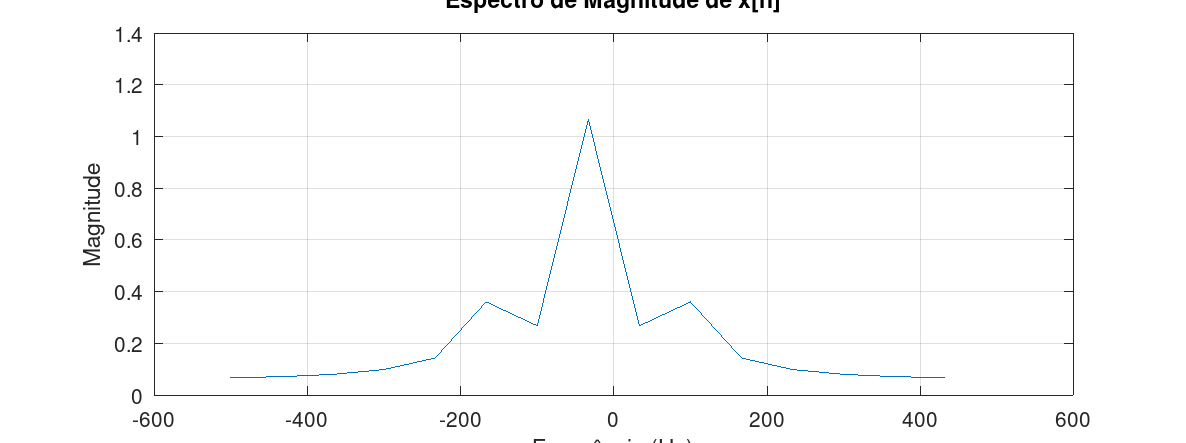
\includegraphics[width=1\linewidth]{03_results/assets/aliasing.png}
    \caption{Espectro com baixo número de amostras.}
    \label{fig:sim-low-sampling}
\end{figure}

Diante dessa situação, surge a pergunta: seria possível ainda reconstruir o sinal? A resposta é sim. Pois, mesmo com o espectro apresentando picos alargados e uma sobreposição parcial devido ao baixo número de amostras, ainda é possível reconstruir o sinal original. Isso ocorre porque:

\begin{enumerate}
    \item Critério de Nyquist foi respeitado: A taxa de amostragem ainda é suficiente para evitar aliasing, o que significa que as frequências do sinal não se confundem com outras frequências espúrias.
    \item Frequências fundamentais são identificáveis: Embora os picos estejam alargados, eles ainda se centram nas frequências corretas, como $\pm 100$ Hz, permitindo identificar as componentes principais do sinal.
    \item Sobreposição parcial não impede a reconstrução: O alargamento dos picos indica baixa resolução espectral, mas enquanto as frequências centrais puderem ser estimadas, o sinal ainda pode ser reconstruído com uma precisão razoável.
    \item Tempo de observação curto impacta resolução, não a existência do sinal: O número limitado de amostras afeta a resolução, mas não altera a presença das frequências fundamentais do sinal.
\end{enumerate}

Em resumo, apesar das limitações de resolução, a informação essencial para a reconstrução do sinal está presente no espectro. Aumentar o número de amostras refinaria a precisão, mas com o espectro atual, a reconstrução ainda é viável, pois as frequências centrais podem ser identificadas com segurança.

% \subsection*{Limitações do Experimento}
% Discutir limitações do experimento
